\documentclass{beamer}
\usepackage{tikz,amsmath,hyperref,graphicx,stackrel,animate,tipa,bm}
\usetikzlibrary{positioning,shadows,arrows,shapes,calc}
\newcommand{\ipa}[1]{\textipa{#1}}
\newcommand{\argmax}{\operatornamewithlimits{argmax}}
\newcommand{\argmin}{\operatornamewithlimits{argmin}}
\mode<presentation>{\usetheme{Frankfurt}}
\DeclareMathOperator*{\softmax}{softmax}
\AtBeginSection[]
{
  \begin{frame}<beamer>
    \frametitle{Outline}
    \tableofcontents[currentsection,currentsubsection]
  \end{frame}
}
\title{Gaussians and Continuous-Density HMMs}
\author{Mark Hasegawa-Johnson\\These slides are in the public domain}
\date{ECE 417: Multimedia Signal Processing}  
\begin{document}

% Title
\begin{frame}
  \maketitle
\end{frame}

% Title
\begin{frame}
  \tableofcontents
\end{frame}

%%%%%%%%%%%%%%%%%%%%%%%%%%%%%%%%%%%%%%%%%%%%
\section[Gaussians]{Gaussians, Brownian motion, and white noise}
\setcounter{subsection}{1}

\begin{frame}
  \frametitle{Gaussian (Normal) pdf}

  \begin{itemize}
  \item Gauss considered this problem: under what circumstances does
    it make sense to estimate the mean of a distribution, $\mu$, by
    taking the average of the experimental values,
    $m=\frac{1}{n}\sum_{i=1}^nx_i$?
  \item He demonstrated that $m$ is the maximum likelihood estimate of
    $\mu$ if (not only if!) $X$ is distributed with the following
    probability density:
  \end{itemize}
  \begin{displaymath}
    p_X(x)=\frac{1}{\sqrt{2\pi\sigma^2}}e^{-\frac{1}{2}\left(\frac{x-\mu}{\sigma}\right)^2}
  \end{displaymath}
\end{frame}


\begin{frame}
  \frametitle{Gaussian pdf}
  \centerline{\includegraphics[height=0.8\textheight]{exp/Boxplot_vs_PDF.png}}
  \url{https://commons.wikimedia.org/wiki/File:Boxplot_vs_PDF.svg}
\end{frame}

\begin{frame}
  \frametitle{Unit Normal pdf}

  Suppose that $X$ is normal with mean $\mu$ and standard deviation
  $\sigma$ (variance $\sigma^2$):
  \begin{displaymath}
    p_X(x) = \mathcal{N}(x;\mu,\sigma^2)=
    \frac{1}{\sqrt{2\pi\sigma^2}}e^{-\frac{1}{2}\left(\frac{x-\mu}{\sigma}\right)^2}
  \end{displaymath}
  Then $U=\left(\frac{X-\mu}{\sigma}\right)$ is normal with mean 0 and
  standard deviation 1:
  \begin{displaymath}
    p_U(u) = \mathcal{N}(u;0,1)=
    \frac{1}{\sqrt{2\pi}}e^{-\frac{1}{2}u^2}
  \end{displaymath}
\end{frame}
  
\begin{frame}
  \frametitle{Central Limit Theorem}

  The Gaussian pdf is important because of the Central Limit Theorem.
  Suppose $X_i$ are i.i.d. (independent and identically distributed),
  each having mean $\mu$ and variance $\sigma^2$.  Then
  \centerline{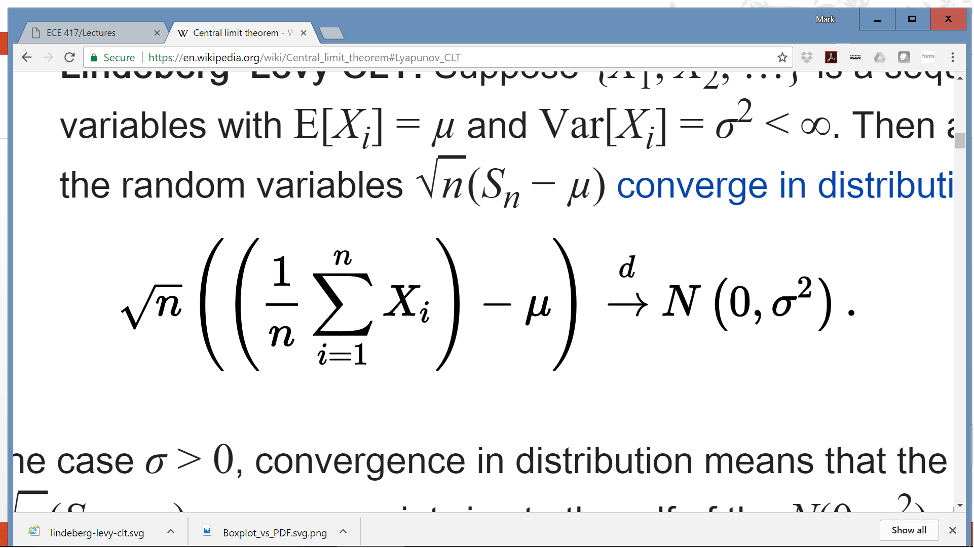
\includegraphics[height=0.5\textheight]{figs/clt.png}}
\end{frame}

\begin{frame}
  \frametitle{Brownian motion}
  \begin{columns}
    \begin{column}{0.5\textwidth}
      The Central Limit Theorem matters because Einstein showed that
      the movement of molecules, in a liquid or gas, is the sum of n
      i.i.d. molecular collisions.

      In other words, the position after $t$ seconds is Gaussian, with
      mean 0, and with a variance of $Dt$, where $D$ is some constant.
    \end{column}
    \begin{column}{0.5\textwidth}
      \centerline{\animategraphics[loop,controls,width=\textwidth]{15}{exp/brownian-}{0}{150}}

      \url{https://commons.wikimedia.org/wiki/File:Brownianmotion5particles150frame.gif}
    \end{column}
  \end{columns}
\end{frame}

\begin{frame}
  \frametitle{White Noise}
  
  \begin{columns}
    \begin{column}{0.5\textwidth}
      \begin{itemize}
        \item Sound = air pressure fluctuations caused by velocity of air molecules
        \item Velocity of warm air molecules without any external sound source = Gaussian
      \end{itemize}
      Therefore:
      \begin{itemize}
      \item Sound produced by warm air molecules without any external sound source = Gaussian noise
      \item Electrical signals: same.
      \end{itemize}
    \end{column}
    \begin{column}{0.5\textwidth}
      \centerline{\includegraphics[width=\textwidth]{exp/White_noise.png}}

      \url{https://commons.wikimedia.org/wiki/File:White_noise.svg}
    \end{column}
  \end{columns}
\end{frame}

\begin{frame}
  \frametitle{White Noise}
  
  \begin{columns}
    \begin{column}{0.5\textwidth}
      \begin{itemize}
        \item White Noise = noise in which each sample of the signal, $x_n$, is i.i.d.
        \item Why ``white''?  Because the Fourier transform,
          $X(\omega)$, is a zero-mean random variable whose variance
          is independent of frequency (``white'')
        \item 
          Gaussian White Noise:
          $x[n]$ are i.i.d. and Gaussian
      \end{itemize}
    \end{column}
    \begin{column}{0.5\textwidth}
      \centerline{\includegraphics[width=\textwidth]{exp/White_noise.png}}

      \url{https://commons.wikimedia.org/wiki/File:White_noise.svg}
    \end{column}
  \end{columns}
\end{frame}


%%%%%%%%%%%%%%%%%%%%%%%%%%%%%%%%%%%%%%%%%%%%
\section[Gaussian Vector]{Gaussian Random Vector}
\setcounter{subsection}{1}

\begin{frame}
  \frametitle{Vector of Independent Gaussian Variables}
  Suppose we have a frame containing $D$ samples from a Gaussian white noise process,
  $x_1,\ldots,x_D$.  Let’s stack them up to make a vector:
  \begin{displaymath}
    \mathbf{x}=\left[\begin{array}{c}x_1\\\vdots\\x_D\end{array}\right]
  \end{displaymath}
  This whole frame is random.  In fact, we could say that $\mathbf{x}$
  is a sample value for a Gaussian random vector called $X$, whose
  elements are $X_1,\ldots,X_D$:
  \begin{displaymath}
    X=\left[\begin{array}{c}X_1\\\vdots\\X_D\end{array}\right]
  \end{displaymath}
\end{frame}

\begin{frame}
  \frametitle{Vector of Independent Gaussian Variables}

  Suppose that the N samples are i.i.d., each one has the same mean,
  $\mu$, and the same variance, $\sigma^2$.  Then the pdf of this
  random vector is
  \begin{displaymath}
    p_X(\mathbf{x}) = \mathcal{N}(\mathbf{x};\bm{\mu},\sigma^2\mathbf{I})=
    \prod_{i=1}^D\frac{1}{\sqrt{2\pi\sigma^2}}e^{-\frac{1}{2}\left(\frac{x_i-\mu}{\sigma}\right)^2}
  \end{displaymath}
\end{frame}

\begin{frame}
  \frametitle{Vector of Independent Gaussian Variables}
  
  \begin{columns}
    \begin{column}{0.5\textwidth}
      Here's an example from Wikipedia with a mean of about 50 and a
      standard deviation of about 12.
    \end{column}
    \begin{column}{0.5\textwidth}
      \centerline{\includegraphics[width=\textwidth]{exp/Multivariate_Gaussian.png}}

      \url{https://commons.wikimedia.org/wiki/File:Multivariate_Gaussian.png}
    \end{column}
  \end{columns}
\end{frame}

\begin{frame}
  \frametitle{Independent Gaussians that aren’t identically distributed}

  Suppose that the N samples are independent Gaussians that aren't
  identically distributed, i.e., $X_i$ has mean $\mu_i$ and variance
  $\sigma_i^2$.  Then the pdf of this random vector is
  \begin{displaymath}
    p_X(\mathbf{x}) = \mathcal{N}(\mathbf{x};\bm{\mu},\mathbf{\Sigma})
    \prod_{i=1}^D\frac{1}{\sqrt{2\pi\sigma_d^2}}e^{-\frac{1}{2}\left(\frac{x_i-\mu_i}{\sigma_i}\right)^2}
  \end{displaymath}
  where $\bm{\mu}$ and $\mathbf{\Sigma}$ are the mean vector and
  covariance matrix:
  \begin{displaymath}
    \bm{\mu}=\left[\begin{array}{c}\mu_1\\\vdots\\\mu_D\end{array}\right],~~~
    \mathbf{\Sigma}=\left[\begin{array}{ccc}\sigma_1^2&0&\cdots\\
        0&\sigma_2^2&\cdots\\\vdots&\vdots&\ddots\end{array}\right]
  \end{displaymath}
\end{frame}

\begin{frame}
  \frametitle{Independent Gaussians that aren’t identically distributed}

  Anpther useful form is:
  \begin{align*}
    p_X(\mathbf{x})
    &=
    \prod_{i=1}^D\frac{1}{\sqrt{2\pi\sigma_d^2}}e^{-\frac{1}{2}\left(\frac{x_i-\mu_i}{\sigma_i}\right)^2}\\
    &=
    \frac{1}{(2\pi)^{D/2}\prod_{i=1}^D\sigma_d}e^{-\frac{1}{2}\sum_{i=1}^d\left(\frac{x_d-\mu_d}{\sigma_d}\right)^2}
  \end{align*}
\end{frame}

\begin{frame}
  \frametitle{Example}

  Suppose that $\mu_1=1$, $\mu_2=-1$, $\sigma_1^2=1$, and
  $\sigma_2^2=4$. Then
  \begin{align*}
    p_X(\mathbf{x})
    &=
    \prod_{i=1}^2\frac{1}{\sqrt{2\pi\sigma_d^2}}e^{-\frac{1}{2}\left(\frac{x_i-\mu_i}{\sigma_i}\right)^2}
    =\frac{1}{4\pi}e^{-\frac{1}{2}\left((x_1-1)^2+\left(\frac{x_2+1}{2}\right)^2\right)}
  \end{align*}
  The pdf has its maximum value, $p_X(\mathbf{x})=\frac{1}{4\pi}$, at
  $\mathbf{x}=\bm{\mu}=\left[\begin{array}{c}1\\-1\end{array}\right]$.
  It drops to $p_X(\mathbf{x})=\frac{1}{4\pi\sqrt{e}}$ at 
  $\mathbf{x}=\left[\begin{array}{c}\mu_1\pm\sigma_1\\\mu_2\end{array}\right]$ and at
  $\mathbf{x}=\left[\begin{array}{c}\mu_1\\\mu_2\pm\sigma_2\end{array}\right]$.
  It drops to $p_X(\mathbf{x})=\frac{1}{4\pi e^2}$ at 
  $\mathbf{x}=\left[\begin{array}{c}\mu_1\pm2\sigma_1\\\mu_2\end{array}\right]$ and at
  $\mathbf{x}=\left[\begin{array}{c}\mu_1\\\mu_2\pm 2\sigma_2\end{array}\right]$.
\end{frame}

\begin{frame}
  \frametitle{Example}
  \centerline{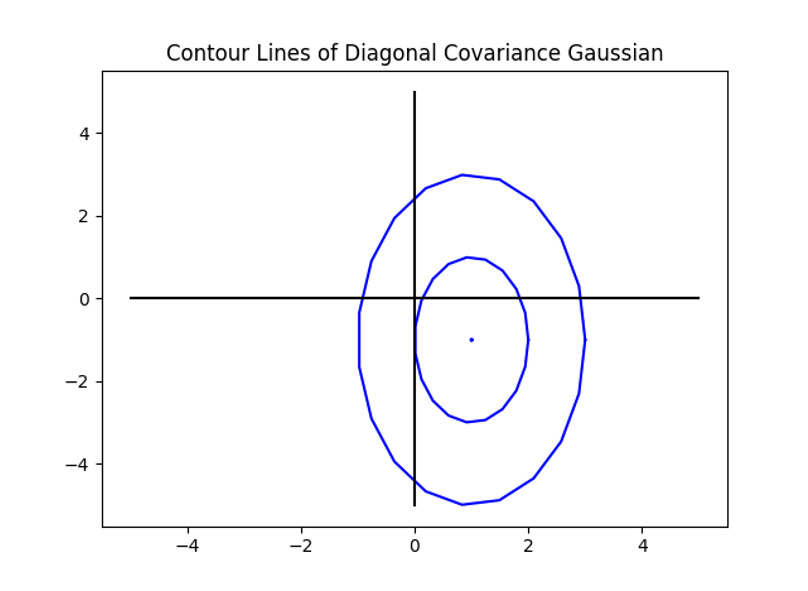
\includegraphics[height=0.8\textheight]{figs/contours_diagonal.png}}
\end{frame}

\begin{frame}
  \frametitle{Facts about linear algebra \#1: determinant of a diagonal matrix}
  Suppose that $\mathbf{\Sigma}$ is a diagonal matrix, with variances on the diagonal:
  \begin{displaymath}
    \mathbf{\Sigma}=\left[\begin{array}{ccc}\sigma_1^2&0&\cdots\\
        0&\sigma_2^2&\cdots\\\vdots&\vdots&\ddots\end{array}\right]
  \end{displaymath}
  Then its determinant is
  \begin{displaymath}
    |\mathbf{\Sigma}| = \prod_{i=1}^D\sigma_d^2
  \end{displaymath}
  So we can write the Gaussian pdf as
  \begin{align*}
    p_X(\mathbf{x})
    =\frac{1}{|2\pi\mathbf{\Sigma}|^{1/2}}e^{-\frac{1}{2}\sum_{i=1}^d\left(\frac{x_d-\mu_d}{\sigma_d}\right)^2}
  \end{align*}
\end{frame}

\begin{frame}
  \frametitle{Facts about linear algebra \#2: inverse of a diagonal matrix}
  Suppose that $\mathbf{\Sigma}$ is a diagonal matrix, with variances on the diagonal:
  \begin{displaymath}
    \mathbf{\Sigma}=\left[\begin{array}{ccc}\sigma_1^2&0&\cdots\\
        0&\sigma_2^2&\cdots\\\vdots&\vdots&\ddots\end{array}\right]
  \end{displaymath}
  Then its inverse is:
  \begin{displaymath}
    \mathbf{\Sigma}^{-1}= \left[\begin{array}{ccc}\frac{1}{\sigma_1^2}&0&\cdots\\
        0&\frac{1}{\sigma_2^2}&\cdots\\\vdots&\vdots&\ddots\end{array}\right]
  \end{displaymath}
\end{frame}

\begin{frame}
  \frametitle{Facts about linear algebra \#3: weighted distance}

  Suppose that
  \begin{displaymath}
    \mathbf{x}=\left[\begin{array}{c}x_1\\\vdots\\x_D\end{array}\right],~~~
    \bm{\mu}=\left[\begin{array}{c}\mu_1\\\vdots\\\mu_D\end{array}\right],~~~
    \mathbf{\Sigma}=\left[\begin{array}{ccc}\sigma_1^2&0&\cdots\\
        0&\sigma_2^2&\cdots\\\vdots&\vdots&\ddots\end{array}\right]    
  \end{displaymath}
  Then
  \begin{align*}
    \sum_{i=1}^D\left(\frac{x_i-\mu_i}{\sigma_i}\right)^2
    &=
        [x_1-\mu_1,x_2-\mu_2,\ldots]
        \left[\begin{array}{ccc}\frac{1}{\sigma_1^2}&0&\cdots\\
            0&\frac{1}{\sigma_2^2}&\cdots\\\vdots&\vdots&\ddots\end{array}\right]
        \left[\begin{array}{c}x_1-\mu_1\\x_2-\mu_2\\\vdots\end{array}\right]\\
        &=(\mathbf{x}-\bm{\mu})^T\mathbf{\Sigma}^{-1}(\mathbf{x}-\bm{\mu})
  \end{align*}
\end{frame}

\begin{frame}
  \frametitle{Mahalanobis distance: Diagonal covariance}

  \begin{columns}
    \begin{column}{0.5\textwidth}
      The Mahalanobis distance between vectors $\mathbf{x}$ and
      $\bm{\mu}$, weighted by covariance matrix $\mathbf{\Sigma}$, is defined to be
      \begin{align*}
        d_{\mathbf{\Sigma}}(\mathbf{x},\bm{\mu}) &=
        \sqrt{(\mathbf{x}-\bm{\mu})^T\mathbf{\Sigma}^{-1}(\mathbf{x}-\bm{\mu})}
      \end{align*}
      If $\mathbf{\Sigma}$ is a diagonal matrix, the Mahalanobis distance is 
      \begin{align*}
        d_{\mathbf{\Sigma}}(\mathbf{x},\bm{\mu}) &=
        \sum_{i=1}^D\left(\frac{x_i-\mu_i}{\sigma_i}\right)^2
      \end{align*}
      The contour lines of equal Mahalanobis distance are ellipses.
    \end{column}
    \begin{column}{0.5\textwidth}
      \centerline{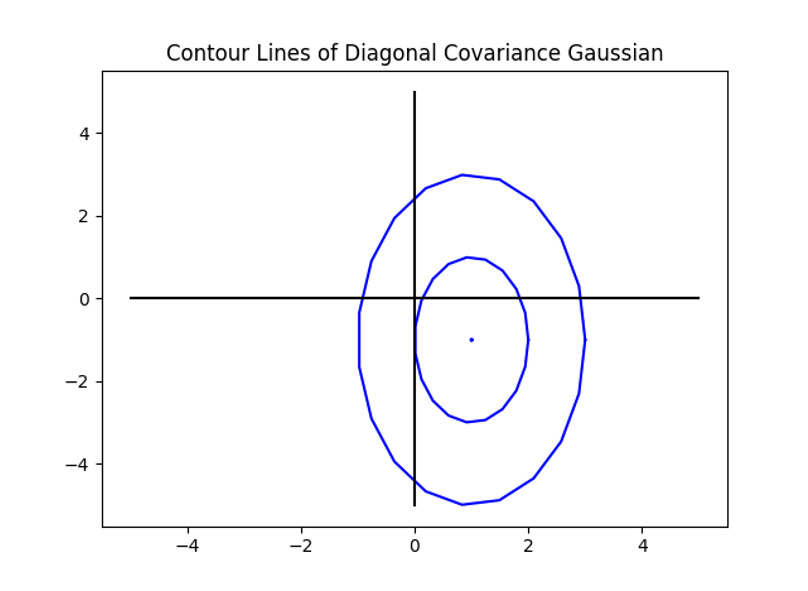
\includegraphics[width=\textwidth]{figs/contours_diagonal.png}}

      \url{https://commons.wikimedia.org/wiki/File:Multivariate_Gaussian.png}
    \end{column}
  \end{columns}
\end{frame}

\begin{frame}
  \frametitle{Independent Gaussians that aren’t identically distributed}

  So if we have independent Gaussians that aren't identically
  distributed, we can write the pdf as
  \begin{align*}
    p_X(\mathbf{x}) &= 
    \frac{1}{(2\pi)^{D/2}\prod_{i=1}^D\sigma_i}e^{-\frac{1}{2}\sum_{i=1}^D\left(\frac{x_i-\mu_i}{\sigma_i}\right)^2}
  \end{align*}
  or as
  \begin{align*}
    p_X(\mathbf{x}) &=
    \frac{1}{|2\pi\mathbf{\Sigma}|^{1/2}}e^{-\frac{1}{2}(\mathbf{x}-\bm{\mu})^T\mathbf{\Sigma}^{-1}(\mathbf{x}-\bm{\mu})}
  \end{align*}
  or as
  \begin{align*}
    p_X(\mathbf{x}) &=
    \frac{1}{|2\pi\mathbf{\Sigma}|^{1/2}}e^{-\frac{1}{2}d_{\mathbf{\Sigma}}^2(\mathbf{x},\bm{\mu})}
  \end{align*}
\end{frame}


%%%%%%%%%%%%%%%%%%%%%%%%%%%%%%%%%%%%%%%%%%%%
\section[HMM]{HMM with Gaussian Observation Probabilities}
\setcounter{subsection}{1}

\begin{frame}
  \frametitle{Review: HMM with Discrete Observations}

  \begin{enumerate}
  \item {\bf Initial State Probabilities:}
    \[
    \pi_i'=\frac{E\left[\mbox{\# state sequences that start with}~q_1=i\right]}{\mbox{\# state sequences in training data}}
    \]
  \item {\bf Transition Probabilities:}
    \[
    \pi_i'=\frac{E\left[\mbox{\# frames in which}~q_{t-1}=i,q_t=j\right]}{E\left[\mbox{\# frames in which}~q_{t-1}=i\right]}
    \]
  \item {\bf Observation Probabilities:} 
    \[
    b_j'(k)=\frac{E\left[\mbox{\# frames in which}~q_t=j,k_t=k\right]}{E\left[\mbox{\# frames in which}~q_{t}=j\right]}
    \]
  \end{enumerate}
\end{frame}

\begin{frame}
  \frametitle{Baum-Welch with Gaussian Probabilities}

  The requirement that we vector-quantize the observations is a
  problem.  It means that we can't model the observations very precisely.

  It would be better if we could model the observation likelihood,
  $b_j(\mathbf{x})$, as a probability density in the space
  $\mathbf{x}\in\Re^D$.  One way is to use a parameterized function that
  is guaranteed to be a properly normalized pdf.  For example, a
  Gaussian:
  \begin{displaymath}
    b_i(\mathbf{x}) = {\mathcal N}\left(\mathbf{x};\bm{\mu}_i,\mathbf{\Sigma}_i\right)
  \end{displaymath}
\end{frame}
  
\begin{frame}
  \frametitle{Diagonal-Covariance Gaussian pdf}

  Let's assume the feature vector has $D$ dimensions,
  $\mathbf{x}_t=[x_{t,1},\ldots,x_{t,D}]$.  The Gaussian pdf is
  \begin{displaymath}
    b_i(\mathbf{x}_t) = 
    \frac{1}{(2\pi)^{D/2}|\mathbf{\Sigma}_i|^{1/2}}e^{-\frac{1}{2}(\mathbf{x}_t-\bm{\mu}_i)\mathbf{\Sigma}_i^{-1}(\mathbf{x}_t-\bm{\mu}_i)^T}
  \end{displaymath}
  The logarithm of a Gaussian is
  \begin{displaymath}
    \ln b_i(\mathbf{x}_t)=
    -\frac{1}{2}\left((\mathbf{x}_t-\bm{\mu}_i)^T\mathbf{\Sigma}_i^{-1}(\mathbf{x}_t-\bm{\mu}_i)
    +\ln|\mathbf{\Sigma}_i| + C\right)
  \end{displaymath}
  where the constant is $C=D\ln(2\pi)$.
\end{frame}

\begin{frame}
  \frametitle{Baum-Welch}

  Baum-Welch maximizes the expected
  log probability, i.e.,
  \begin{displaymath}
    E_{\mathbf{q}|\mathbf{X}}\left[\ln b_i(\mathbf{x}_t)\right]=
    -\frac{1}{2}\sum_{i=1}^N \gamma_t(i)\left(
    (\mathbf{x}_t-\bm{\mu}_i)^T\mathbf{\Sigma}_i^{-1}(\mathbf{x}_t-\bm{\mu}_i)
    +\ln|\mathbf{\Sigma}_i|+C\right)
  \end{displaymath}
  If we include all of the frames, then we get
  \begin{align*}
    &E_{\mathbf{q}|\mathbf{X}}\left[\ln p(\mathbf{X},\mathbf{q}|\Lambda)\right] = \mbox{other terms}\\
    &-\frac{1}{2}\sum_{t=1}^T \sum_{i=1}^N \gamma_t(i)\left(
    (\mathbf{x}_t-\bm{\mu}_i)^T\mathbf{\Sigma}_i^{-1}(\mathbf{x}_t-\bm{\mu}_i)
    +\ln|\mathbf{\Sigma}_i|+C\right) 
  \end{align*}
  where the ``other terms'' are about $a_{i,j}$ and $\pi_i$, and have
  nothing to do with $\bm{\mu}_i$ or $\mathbf{\Sigma}_i$.
\end{frame}
  
\begin{frame}
  \frametitle{M-Step: optimum $\bm{\mu}$}

  First, let's optimize $\bm{\mu}$.  We want
  \begin{displaymath}
    0 = \frac{\partial}{\partial{\bm{\mu}_q}}\sum_{t=1}^T\sum_{i=1}^N\gamma_t(i)(\mathbf{x}_t-\bm{\mu}_i)^T\mathbf{\Sigma}_i^{-1}(\mathbf{x}_t-\bm{\mu}_i)
  \end{displaymath}
  Re-arranging terms, we get
  \begin{displaymath}
    \bm{\mu}_q' = \frac{\sum_{t=1}^T\gamma_t(q)\mathbf{x}_{t}}{\sum_{t=1}^T\gamma_t(q)}
  \end{displaymath}
\end{frame}

\begin{frame}
  \frametitle{M-Step: optimum $\mathbf{\Sigma}$}

  Second, let's optimize $\mathbf{\Sigma}_{i}$.
  For this, it's easier to express the log likelihood as
  \begin{align*}
    E_{\mathbf{q}|\mathbf{X}}\left[\ln p_X(\mathbf{X},\mathbf{q})\right] &=\mbox{other stuff}
    -\frac{1}{2}\sum_{t=1}^T\gamma_t(i)
    \sum_{d=1}^D\left(\ln\sigma_{i,d}^2+\frac{(x_{t,d}-\mu_{i,d})^2}{\sigma_{i,d}^2}\right)
  \end{align*}
  Its scalar derivative is
  \begin{align*}
    \frac{\partial E_{\mathbf{q}|\mathbf{X}}\left[\ln p_X(\mathbf{X},\mathbf{q})\right]}{\partial\sigma_{i,d}^2} &=
    -\frac{1}{2}\sum_{t=1}^T\gamma_t(i)\left(\frac{1}{\sigma_{i,d}^2}-\frac{(x_{t,d}-\mu_{i,d})^2}{\sigma_{i,d}^4}\right)
  \end{align*}
  Which we can solve to find
  \begin{align*}
    \sigma_{i,d}^2 = \frac{\sum_{t=1}^T\gamma_t(i)(x_{t,d}-\mu_{t,d})^2}{\sum_{t=1}^T\gamma_t(i)}
  \end{align*}
\end{frame}
  
  
\begin{frame}
  \frametitle{Minimizing the cross-entropy: optimum $\sigma$}

  Arranging all the scalar derivatives into a matrix, we can write
  \begin{displaymath}
    \mathbf{\Sigma}_{i}' = \frac{\sum_{t=1}^T\gamma_t(i)(\mathbf{x}_{t}-\bm{\mu}_{i})(\mathbf{x}_t-\bm{\mu}_i)^T}{\sum_{t=1}^T\gamma_t(i)}
  \end{displaymath}
  \begin{itemize}
    \item 
      Actually, the above formula holds even if the Gaussian has a
      non-diagonal covariance matrix, but Gaussians with non-diagonal
      covariance matrices work surprisingly badly in HMMs.
    \item
      For a diagonal-covariance Gaussian, we evaluate only the
      diagonal elements of the vector outer product
      $(\mathbf{x}_{t}-\bm{\mu}_{i})(\mathbf{x}_t-\bm{\mu}_i)^T$
  \end{itemize}
\end{frame}

\begin{frame}
  \frametitle{Summary: Gaussian Observation PDFs}

  So we can use Gaussians for $b_j(\mathbf{x})$:
  \begin{itemize}
  \item {\bf E-Step:}
    \[
    \gamma_t(i) = \frac{\alpha_t(i)\beta_t(i)}{\sum_{i'}\alpha_t(i')\beta_t(i')}
    \]
  \item {\bf M-Step:}
    \begin{displaymath}
      \bm{\mu}_{i}' = \frac{\sum_{t=1}^T\gamma_t(i)\mathbf{x}_{t}}{\sum_{t=1}^T\gamma_t(i)}
    \end{displaymath}
    \begin{displaymath}
      \mathbf{\Sigma}_{i}' = \frac{\sum_{t=1}^T\gamma_t(i)(\mathbf{x}_{t}-\bm{\mu}_{i})(\mathbf{x}_t-\bm{\mu}_i)^T}{\sum_{t=1}^T\gamma_t(i)}
    \end{displaymath}
  \end{itemize}
\end{frame}

%%%%%%%%%%%%%%%%%%%%%%%%%%%%%%%%%%%%%%%%%%%%
\section[Summary]{Summary}
\setcounter{subsection}{1}

\begin{frame}
  \frametitle{Summary: Independent Gaussians that aren’t identically distributed}

  \begin{align*}
    p_X(\mathbf{x}) &= 
    \frac{1}{(2\pi)^{D/2}\prod_{i=1}^D\sigma_i}e^{-\frac{1}{2}\sum_{i=1}^D\left(\frac{x_i-\mu_i}{\sigma_i}\right)^2}
    \\
    &=
    \frac{1}{|2\pi\mathbf{\Sigma}|^{1/2}}e^{-\frac{1}{2}(\mathbf{x}-\bm{\mu})^T\mathbf{\Sigma}^{-1}(\mathbf{x}-\bm{\mu})}\\
    &=
    \frac{1}{|2\pi\mathbf{\Sigma}|^{1/2}}e^{-\frac{1}{2}d_{\mathbf{\Sigma}}^2(\mathbf{x},\bm{\mu})}
  \end{align*}
\end{frame}

\begin{frame}
  \frametitle{Summary: Gaussian Observation PDFs}

  So we can use Gaussians for $b_j(\mathbf{x})$:
  \begin{itemize}
  \item {\bf E-Step:}
    \[
    \gamma_t(i) = \frac{\alpha_t(i)\beta_t(i)}{\sum_{i'}\alpha_t(i')\beta_t(i')}
    \]
  \item {\bf M-Step:}
    \begin{displaymath}
      \bm{\mu}_{i}' = \frac{\sum_{t=1}^T\gamma_t(i)\mathbf{x}_{t}}{\sum_{t=1}^T\gamma_t(i)}
    \end{displaymath}
    \begin{displaymath}
      \mathbf{\Sigma}_{i}' = \frac{\sum_{t=1}^T\gamma_t(i)(\mathbf{x}_{t}-\bm{\mu}_{i})(\mathbf{x}_t-\bm{\mu}_i)^T}{\sum_{t=1}^T\gamma_t(i)}
    \end{displaymath}
  \end{itemize}
\end{frame}


\end{document}

